\documentclass[a4paper,twoside,10pt]{article}
\usepackage{tutorial}
\graphicspath{{figs/}}
\def\figurename{Figure}
\def\tablename{Tableau}
\newcommand{\italic}[1]{\emph{#1}} 

% ------------------------------------------------------------------------
\newcommand\IL{{\itshape left}}
\newcommand\IR{{\itshape right}}
\newcommand\IM{{\itshape middle}}
\newcommand\IT{{\itshape top}}
\newcommand\IB{{\itshape bottom}}

% ------------------------------------------------------------------------
\def\kernel{\lstinline!Kernel!}

\def\cgalpoly{\lstinline!CGAL::Polyhedron_3!}
\def\poly{\lstinline!Polyhedron_3!}
\def\polytrait{\lstinline!PolyhedronTraits_3!}
\def\polyitem{\lstinline!PolyhedronItems_3!}
\def\polybuilder{\lstinline!Polyhedron_incremental_builder_3!}

\def\cgalhds{\lstinline!CGAL::HalfedgeDS!}
\def\hds{\lstinline!HalfedgeDS!}
\def\hdsitem{\lstinline!PolyhedronItems!}


\newcommand{\CodeFmt}[1]{{\small\texttt{#1}}}
\def\cgalpoly{\CodeFmt{Polyhedron\_3}}


% hyperref stuff
\usepackage{hyperref}
\hypersetup{
  pdftitle={Getting started with CGAL Polyhedron},
  pdfauthor={INRIA Geometrica},
  pdfsubject={A tutorial for CGAL},
  pdfkeywords={},
  pdfpagemode=UseThumbs,
  baseurl={http://www.cgal.org},
  colorlinks=true,
  linkcolor=black,
  anchorcolor=black,
  citecolor=black,
  filecolor=black,
  menucolor=black,
  pagecolor=black,
  urlcolor=blue,
  bookmarksopen=false,}
% end hyperref stuff


\begin{document}

% TITLE
\date{}
\title{{\LARGE {\sffamily\bfseries Getting started with CGAL
Polyhedron}}\\ the example of subdivision surfaces}
\author{
\sffamily Pierre Alliez\footnote{GEOMETRICA, INRIA Sophia-Antipolis}
\and 
\sffamily Andreas Fabri\footnote{GeometryFactory, Sophia-Antipolis}
\and 
\sffamily Lutz Kettner\footnote{Max-Planck Institut f�r Informatik, 
                                Saarbr�cken}
\and
\sffamily Le-Jeng Shiue\footnote{SurfLab, University of Florida}
\and
\sffamily Radu Ursu\footnote{GEOMETRICA, INRIA Sophia-Antipolis}}
\maketitle

\thispagestyle{empty}

% ABSTRACT

\abstract{This document gives a description for a user to get
started with the halfedge data structure provided by the Computational
Geometry Algorithm Library (CGAL). Assuming the reader to be familiar
with the C++ template mechanisms and the key concepts of the Standard
Template Library (STL), we describe three different approaches with
increasing level of sophistication for implementing mesh subdivision
schemes. The simplest approach uses simple Euler operators to
implement the $\sqrt{3}$ subdivision scheme applicable to triangle
meshes. A second approach overloads the incremental builder already
provided by CGAL to implement the quad-triangle subdivision scheme
applicable to polygon meshes. The third approach is more generic and
offers an efficient way to design its own subdivision scheme through
the definition of rule templates. Catmull-Clark, Loop and Doo-Sabin
schemes are illustrated using the latter approach. Two companion
applications, one developed on Windows with MS .NET, MFC and OpenGL,
and the other developed for both Linux and Windows with Qt and OpenGL,
implement the subdivision schemes listed above, as well as several
functionalities for interaction, visualization and raster/vectorial
output.}

\vskip 3mm

\noindent {\bf Keywords:}
                 CGAL library,
                 tutorial, 
                 halfedge data structure, 
                 polygon surface mesh,
                 subdivision surfaces,
                 quad-triangle subdivision scheme,
                 $\sqrt{3}$,
                 Loop,
                 Doo-Sabin,
                 Catmull-Clark,
                 OpenGL.

% INTRODUCTION                 
\section{Introduction}

% introduction to cgal

The CGAL library is a joint effort between nine European
institutes~\cite{fgkss-dccga-00}. The goal of CGAL is to make
available to users in industry and academia the most important
efficient solutions to basic geometric problems developed in the area
of computational geometry in a C++ software library.\\

% motivations

CGAL features a 3D polygon surface mesh data structure based on the
concept of halfedge data structure~\cite{k-ugpdd-99}, which has been
very successful for the design of general algorithms on meshes. In
this document we provide a tutorial to get started with CGAL
Polyhedron data structure through the example of subdivision
surfaces. We also offer an application both under windows and linux,
featuring an OpenGL-based viewer, an arcball for interaction and two
raster and vectorial output to produce pictures and figures.\\

% teaser

\begin{figure}[htb]
    \centering{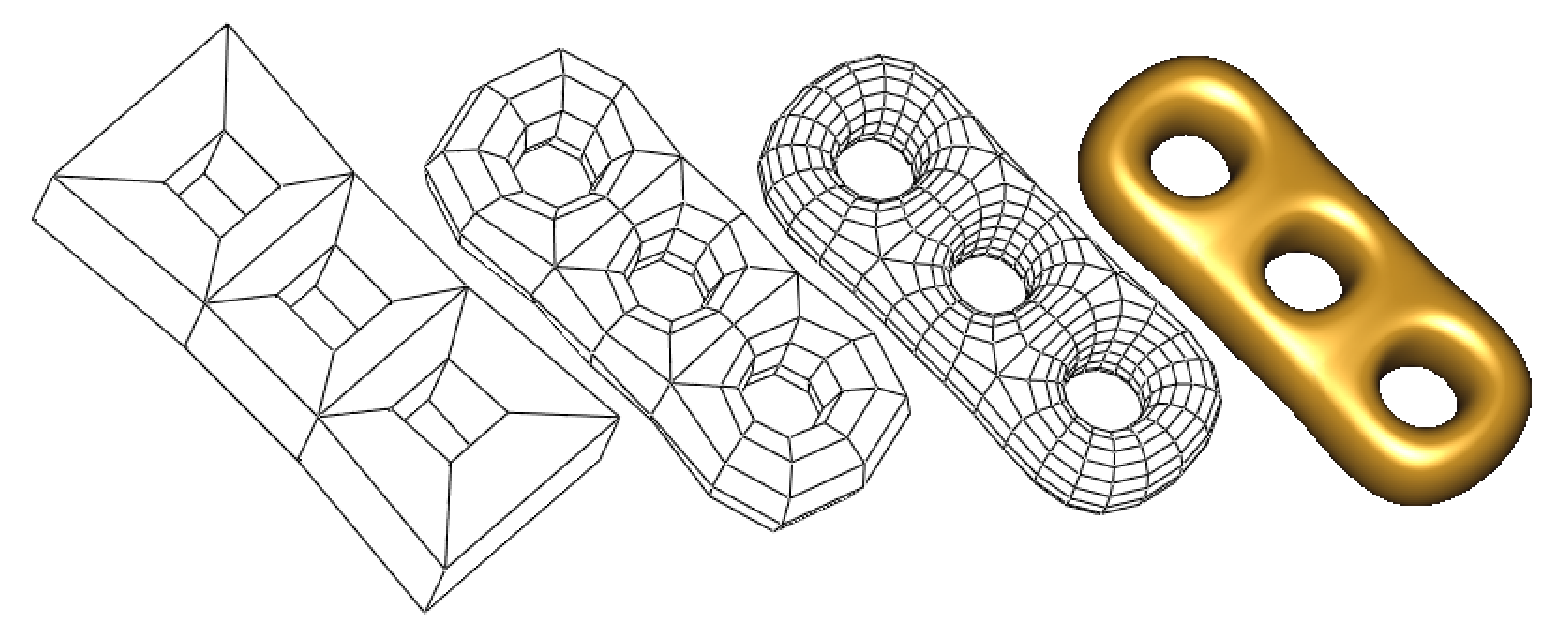
\includegraphics[width=\linewidth]{figs/teaser}}
    \caption{Snapshot taken from the tutorial application running
             on Windows. A polygon mesh is subdivided using the
             quad-triangle subdivision scheme.}
    \label{fig:teaser}
\end{figure}
        

% targeted audience ?

The main targeted audience is a master or Ph.D. student in computer
graphics or computational geometry, aiming at working on mesh
processing algorithms. We hope this tutorial will convince the
reader~:
\begin{itemize}

\item 
not reinventing the wheel. Taking some time choosing the ``right
tool'' is often worth it, even for a short project;

\item 
using an optimized and robust library to ease the implementation and
obtain fast and robust results;

\item 
using generic programming to reuse existing data structures
and algorithms;

\item 
using a standard library in order to benefit from existing support and
discussion groups\footnote{see the cgal discuss list:
\href{http://www.cgal.org/user_support.html}
{http://www.cgal.org/user\_support.html.}}.

\end{itemize}               

% PREREQUISITES
\section{Prerequisites}

% C++ and generic programming

Before using CGAL, it is mandatory to be familiar with C++ and the
\italic{generic programming paradigm}. The latter features the notion
of C++ class templates and function templates, which is at the corner
stone of all features provided by CGAL.

% STL

An excellent example illustrating generic programming is the Standard
Template Library (STL). Generality and flexibility is achieved with a
set of \italic{concepts}, where a concept is a well defined set of
requirements. One of them is the \italic{iterator} concept, which
allows both referring to an item and traversing a sequence of
items. Those items are stored in a data structure called
\italic{container} in STL. Another concept, so-called
\italic{circulator}, allows traversing some circular sequences. They
share most of the requirements with iterators, except the lack of
past-the-end position in the sequence. Since CGAL is strongly inspired 
from the genericity of STL, it is important to become familiar with
its concepts before starting using it (ref STL).

% HALFEDGE DATA STRUCTURE
\section{Halfedge data structure}

The specification of a polygon surface mesh consists of combinatorial
entities: vertices, edges, and faces, and numerical quantities:
attributes such as vertex positions, vertex normals, texture
coordinates, face colors, etc. The \italic{connectivity} describes the
incidences between elements and is implied by the topology of the
mesh. For example, two vertices or two faces are adjacent if there
exists an edge incident to both.\\


% definition

A \italic{halfedge data structure} is an edge-centered data structure
capable of maintaining incidence informations of vertices, edges and
faces, for example for planar maps, polyhedra, or other orientable,
two-dimensional surfaces embedded in arbitrary dimension. Each edge is
decomposed into two halfedges with opposite orientations. One incident
face and one incident vertex are stored in each halfedge. For each
face and each vertex, one incident halfedge is stored (see
Fig.\ref{fig:halfedge}).

% halfedge

\begin{figure}[htb]
    \centering{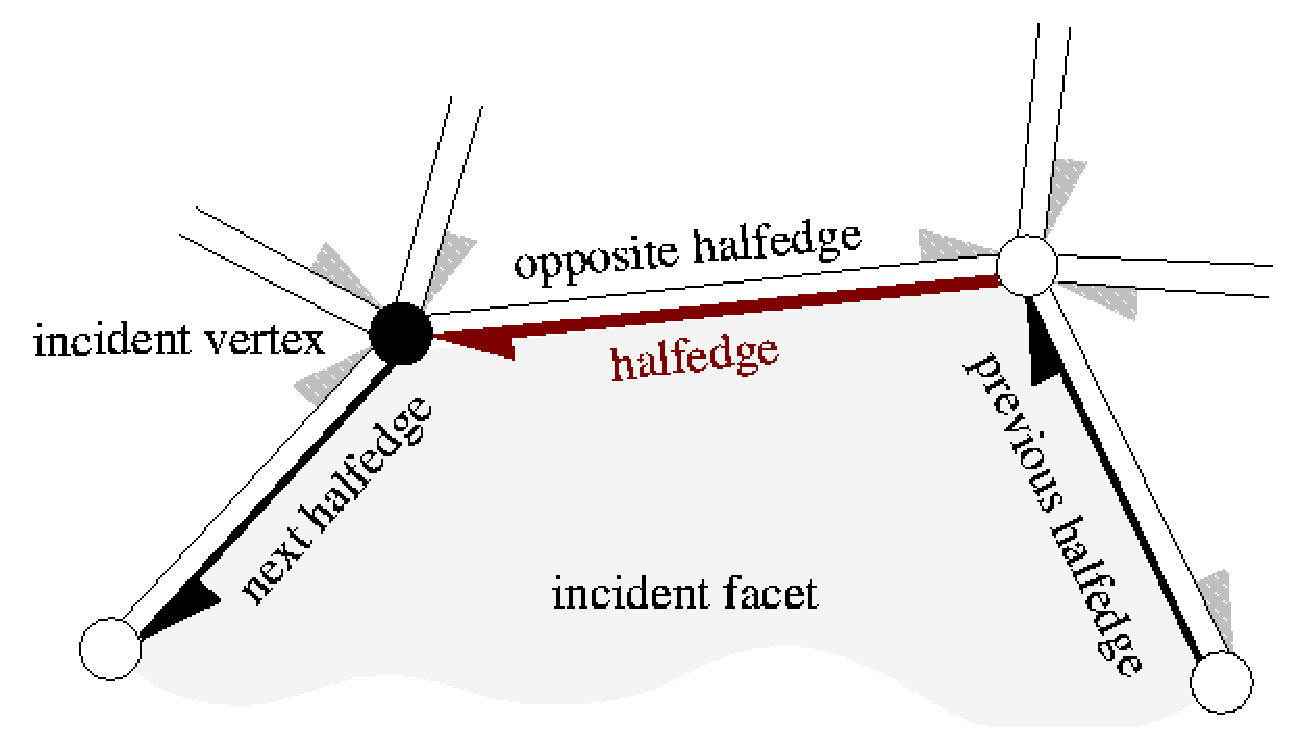
\includegraphics[width=\linewidth]{figs/halfedge}}
    \caption{Halfedge.}  
    \label{fig:halfedge}
\end{figure}
        
Notice that the halfedge data structure is only a combinatorial data
structure, geometric interpretation being added by classes built on
top of the halfedge data structure. On example is the class
\italic{CGAL::Polyhedron\_3} that we use in this tutorial. The 
halfedge data structure has been very successful for the design of
algorithms on meshes for several reasons:

\begin{itemize}

\item 
an edge-based data structure leads to a constant size structure,
contrary to face-based data structures with inevitable variable
topological structure when dealing with arbitrary vertex valence and
face degrees.

\item 
a halfedge encodes the orientation of an edge, facilitating the mesh
traversal.

\item 
navigation around each vertex by visiting all surrounding edges or
faces is made easy.

\item
each halfedge can be associated with a unique corner, that is a couple
$\{$face,vertex$\}$. The storage of attributes such as normals or
texture coordinates per corner (instead of per vertex) is thus
allowed.

\end{itemize}

% STL CONCEPTS APPLIED TO MESHES
\section{STL concepts applied to meshes}

Concepts of iterators and circulators on a mesh.

Circulation around vertices, inside facets, along a boundary.


% POLYHEDRON DATA STRUCTURE
\section{Polyhedron data structure}

Description.

Example of declaration (equipped with a kernel).

Enrich primitives.

Euler operators.

Examples of iteration and circulation.

Incremental builder.

% SUBDIVISION SURFACES
\section{Subdivision surfaces}

A subdivision surface is the limit surface resulting from the
application of a \italic{subdivision scheme} to a control polyhedron
(see Fig.\ref{fig:subdivision}). During this process the polygon base
mesh is recursively subdivided and the mesh geometry is progressively
modified according to subdivision rules. A subdivision scheme is
characterized by a refinement operator that acts on the connectivity
by subdividing the mesh, and by a smoothing operator that modifies the
geometry. We choose the example of subdivision to illustrate (i)
iteration and circulation on a halfedge data structure, (ii)
modification of the connectivity, and (iii) modification of the
geometry.

% subdivision paradigm

\begin{figure}[htb]
    \centering{\includegraphics[width=\linewidth]{figs/subdivision}}
    \caption{Catmull-Clark subdivision of a quadrilateral control mesh.}  
    \label{fig:subdivision}
\end{figure}


\subsection{$\sqrt{3}$-Subdivision using Euler Operators}

The $\sqrt{3}$ subdivision scheme was introduced by
Kobbelt~\cite{k-sqrt3-00}. It takes as input a triangle mesh and
subdivide each facet into three triangles by splitting it at its
centroid. Next, all edges of the initial mesh are flipped so that they
join two adjacent centroids. Finally, each initial vertex is replaced
by a barycentric combination of its neighbors. An example of one step
of the $\sqrt{3}$ subdivision scheme is shown in
Fig.\ref{fig:sqrt3_basic}, and an example of several steps is shown in
Fig.\ref{fig:sqrt3}.

% sqrt3 subdivision (basic)

\begin{figure}[htb]
    \centering{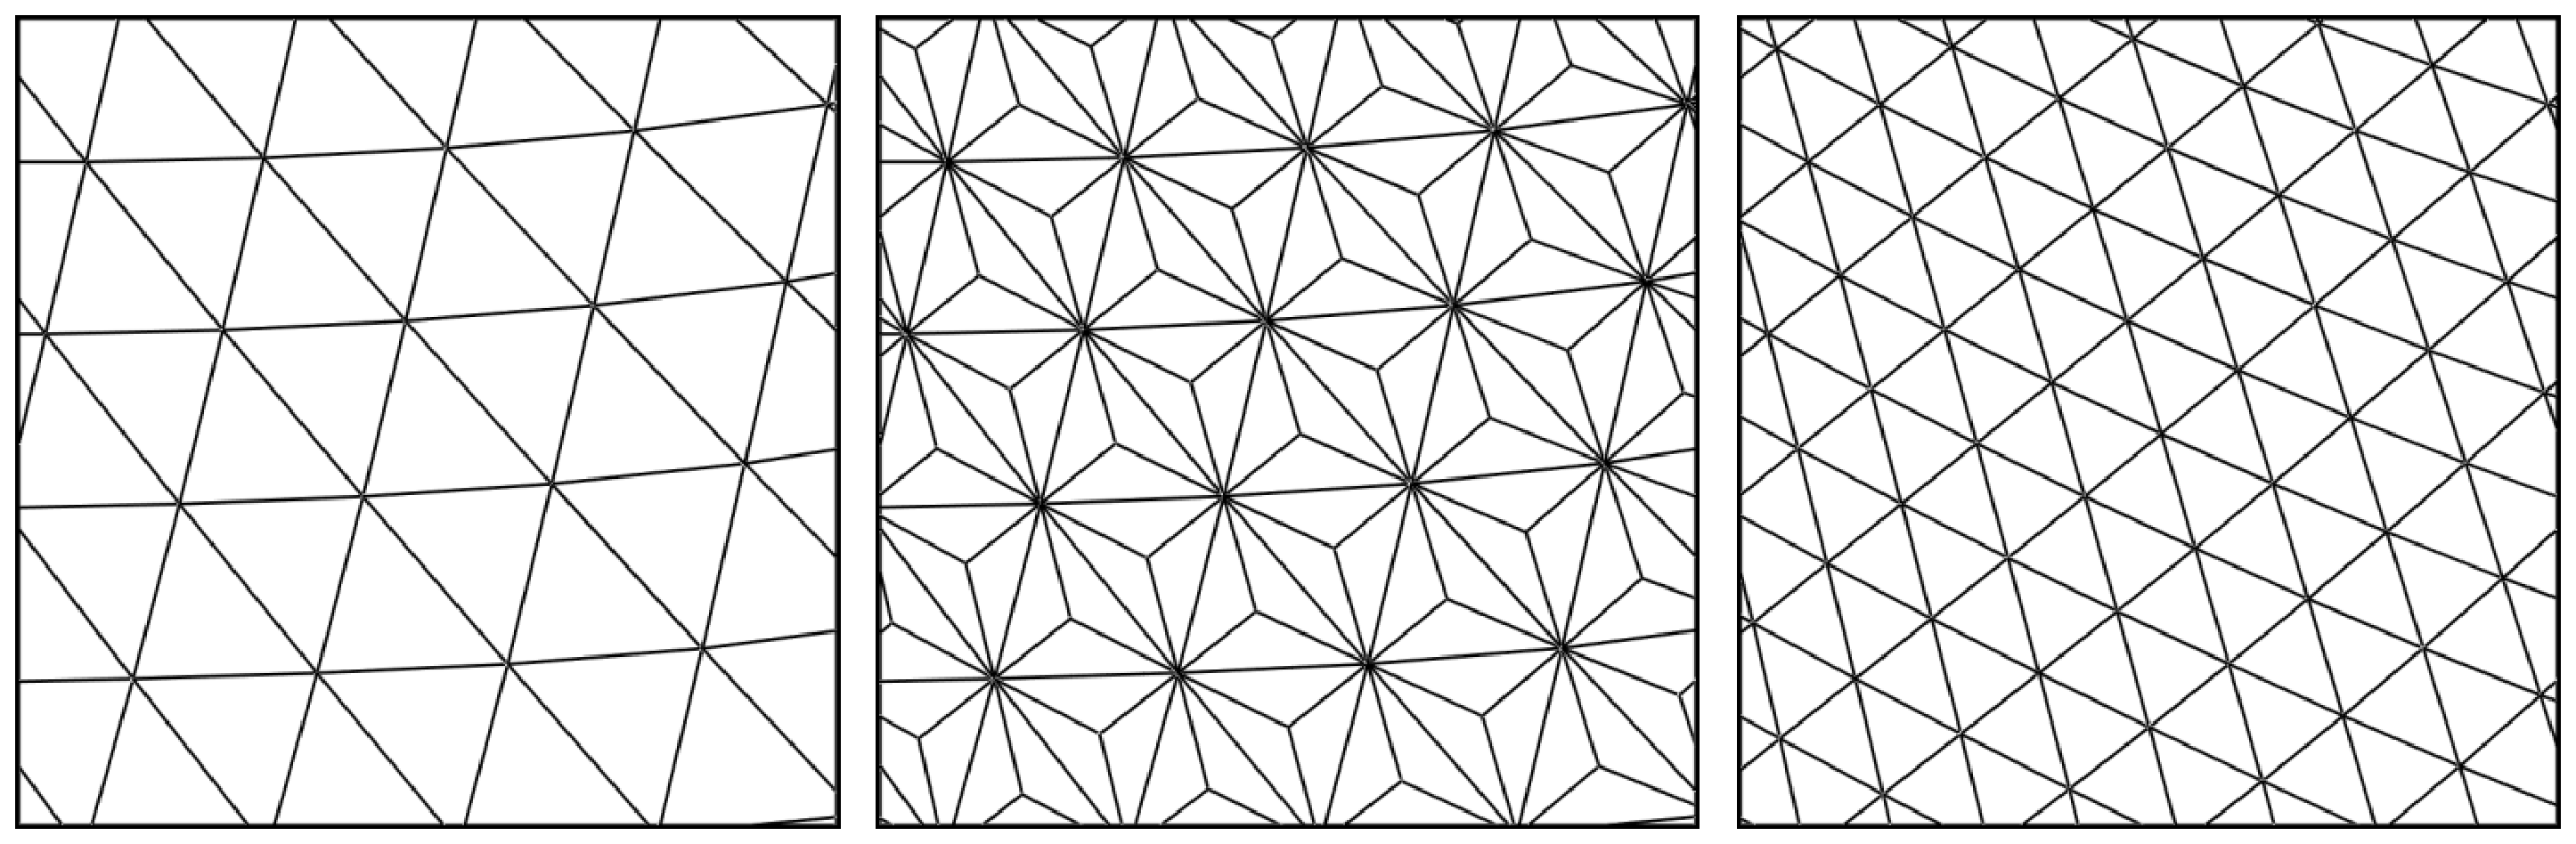
\includegraphics[width=\linewidth]{figs/sqrt3_basic}}
    \caption{The $\sqrt{3}$-Subdivision scheme is decomposed as
             a set of Euler operators: face splits and edge flips.}
    \label{fig:sqrt3_basic}
\end{figure}

% sqrt3 subdivision 

\begin{figure}[htb]
    \centering{\includegraphics[width=\linewidth]{figs/sqrt3}}
    \caption{$\sqrt{3}$-Subdivision of the mannequin mesh.}
    \label{fig:sqrt3}
\end{figure}


\subsection{Quad-triangle Subdivision using Incremental Builder}

The quad-triangle subdivision scheme was introduced by
Levin~\cite{l-pg-03}, then Stam and Loop~\cite{sl-qts-02}. It applies
to polygon meshes and basically features Loop subdivision on triangles
and Catmull-Clark subdivision on polygons of the control mesh (see
Fig.\ref{fig:quad-triangle}). After one iteration of subdivision the
subdivided model is only composed of triangles and quads. A simple
solution for implementing such a scheme is to use the
\italic{incremental builder} concept featured by CGAL Polyhedron. The 
utility class \italic{CGAL::Polyhedron\_incremental\_builder\_3} helps
in creating polyhedral surfaces from a list of vertices followed by a
list of facets that are represented as indices into the vertex
list. This is usually of particular interest for implementing file
readers for common file formats, and we use it here for generating a
subdivided mesh starting from a coarser initial mesh.


% quad-triangle subdivision scheme

\begin{figure}[htb]
    \centering{\includegraphics[width=\linewidth]{figs/quad-triangle}}
    \caption{Quad-triangle subdivision scheme.}
    \label{fig:quad-triangle}
\end{figure}

Subdivision engine

{ \scriptsize
\begin{verbatim}
template <class Polyhedron,class kernel>
class CSubdivider_quad_triangle
{
public:
    typedef typename Polyhedron::HalfedgeDS HalfedgeDS;

public:
  // life cycle
  CSubdivider_quad_triangle() {}
  ~CSubdivider_quad_triangle() {}

public:
  void subdivide(Polyhedron &OriginalMesh,
                 Polyhedron &NewMesh,
                 bool smooth_boundary = true)
  {
    CModifierQuadTriangle<HalfedgeDS,Polyhedron,kernel> 
      builder(&OriginalMesh);

    // delegate construction 
    NewMesh.delegate(builder);

    // smooth
    builder.smooth(&NewMesh,smooth_boundary);
  }
};
\end{verbatim}}

Subdivision using a modified incremental builder

{ \scriptsize
\begin{verbatim}
template <class HDS,class Polyhedron,class kernel>
class CModifierQuadTriangle : public CGAL::Modifier_base<HDS>
{
private:
  Polyhedron *m_pMesh;
  typedef typename CGAL::Enriched_builder<HDS> builder;

public:

  // life cycle
  CModifierQuadTriangle(Polyhedron *pMesh)
  {
    m_pMesh = pMesh;
  }
  ~CModifierQuadTriangle() {}

  // subdivision
  void operator()( HDS& hds)
  {
    builder B(hds,true);
    B.begin_surface(3,1,6);
      add_vertices(B);
      add_facets(B);
    B.end_surface();
  }
...
};
\end{verbatim}}




% SurfLab

\subsection{Subdivision using a rule template}

Doo-Sabin, Catmull-Clark, Loop.

% APPLICATION DEMO
\section{Application demo}

List of features, snapshots.

\subsection{Compiling on Windows}

\subsection{Compiling on Linux}

% CONCLUSION
\section{Conclusion}

% REFERENCES
\bibliographystyle{alpha}
\bibliography{tutorial}


\end{document}
